\chapter{Cryptography}
	\label{ch:Cryptography}
		%Resource: http://www.thegeekstuff.com/2012/07/cryptography-basics/
		%Resource: http://www.pgpi.org/doc/pgpintro/
		%Resource: http://cacr.uwaterloo.ca/hac/
		Cryptography is the closest means of securely transmitting data across a network that is currently available. 
		It is also the only means of ensuring that data cannot be read by any individual who has access to a storage medium. 
		Thus, it is one of the more important concepts in computational security. 
		Without cryptography, nothing can be confirmed and nothing is secure. 
		However, cryptography is something that is easy to get wrong.
		It can be hard to ensure all minor steps are followed, but missing only one will lead to significant weaknesses. 
		This section will discuss the basic ideas of cryptography without the mathematical background or the algorithmic understanding. 
		It will provide an overview on the requirements for a secure transmission. 
		The technical details of this will be presented in the later sections of this chapter. 
		These details for the specific standards that are used later in this chapter can be found in the FIPS released by NIST.\footnote{\url{http://csrc.nist.gov/groups/STM/cmvp/index.html}}
		Furthermore, if you wish to understand the mathematical background, I suggest further reading such as Schnier's \textit{Applied Cryptography}\cite{ACrypto}.
	\section{Introduction to Cryptography}
		This section will outline the basic ideas that one must understand before they can delve into deeper cryptography. 
		It will first discuss the terminology that is used in the area, followed by a basic outline of cryptographical types and early implementations. 
		\subsection{Key Terms}
			There are a number of terms within Cryptography that you will need to understand before you will understand the field.
			These terms are used to explain the goal or use of a particular part of cryptography\footnote{\url{http://www.thegeekstuff.com/2012/07/cryptography-basics/}}
			\begin{description}
				\item[Plaintext]
					The original message that is to be sent, signed or checked. 
					This is the message that the user or protocol writes to be transmitted to the other host or stored. 
				\item[Ciphertext]
					This is the cryptographically ``secure'' form of the plaintext above. 
					This means that the plaintext has gone through a cryptographical algorithm and is now enciphered within this text. 
				\item[Code] A substitution of words to generate a ciphertext. 
					This was (and still often is) used in military communications to throw off the enemy. 
					It could replace a phrase such as ``attack at dawn'' with ``Ocelot'', leading to confusion without the code. 
				\item[Cipher] A means of cryptography which unlike the code above is general. 
					This means that it can be used on any word or phrase without first creating a codebook. 
					This is the means of cryptography this chapter will discuss.
				\item[Encryption]
					Conversion from a readable plaintext into an unreadable ciphertext. 
					This is mainly used to gain privacy in either storage or transmission. 
					This process will also come with a key or key pair that is used to encrypt the plaintext. 
				\item[Decryption]
					The process of converting an unreadable ciphertext into a readable plaintext. 
					This is used to allow the decrypting party to read the text. 
					This process will also need either the key, or the second half of the key pair. 
				\item[Authentication]
					This is the act of ensuring that the message received came from the sender claimed by the message. 
					This is based on an action that the receiving party knows only the sending party should be able to do. 
					Usually, this is done through signing with a private key. 
					The signature is then checked with the public key. 
				\item[Integrity] 
					This is the process of checking that the message received has not been altered in transmission. 
					This check is done on receipt of the message, ensuring that any changes in transmission are noticed. 
					Hashing algorithms such as SHA and MD5 are usually used for this process. 
				\item[Non-repudiation]
					Messages that are sent can be traced back to the original source. 
					That source cannot say that they did not send the message as a digital signature has stated their action. 
					This is done in much the same manner as authentication. 
				\item[Hash]
					This is a ``one way'' algorithm that takes a message an converts in into another form. 
					The basis of this is that there should be no way to reverse the algorithm given the output hash. 
					Furthermore, there should be minimal collisions with other messages. 
				\item[Algorithm] Also known as a cipher, is the mathematical function used for encryption and decryption. 
					If the security of the algorithm is based on it's secrecy, it is known as a restricted algorithm. 
					However, most modern algorithms are open standards as knowing the algorithm does not help without the key. 
				\item[Key] The string or data used by a non-restricted algorithm to encrypt or decrypt. 
					This is the part of the process that must be held secure in modern cryptography. 
				\item[KDC] Key Distribution Centre. 
					This is the place that public keys are stored for later access by other parties. 
					It is used to ensure that the correct public key is released by signing for the authenticity of each key. 
				\item[Symmetric Algorithm] The same key is used for both encryption and decryption. 
					Generally, this is faster, but has the problem of key transmission. 
					This will be covered in greater depth later in this section. 
				\item[Asymmetric Algorithm] Two different keys are used in the encryption and decryption process. 
					Each user is given their partners public key, which is used for encryption. 
					The receiving partner can then decrypt using their private key. 
					This will be further explained later in this section. 
				\item[Cryptanalysis] The process of reverse engineering a cryptographical solution in an attempt to attack the ciphertext to gain the plaintext. 
					In this, it is generally assumed that the analyst has access to the full algorithm, but not the key. 
					There are four types of cryptanalysis: 
					\begin{enumerate}
						\item \textbf{Ciphertext only:} The attacker has the ciphertext of several messages using the same algorithm. 
							This is an attempt to deduce the plain text or key used. 
						\item \textbf{Known Plaintext:} The attacker has access to both ciphertext and plaintext. 
							The goal here is to deduce the key given a cipher-plain text pair. 
						\item \textbf{Chosen plaintext:} The attacker is creating a custom plaintext. 
							This is useful as some plaintext blocks provide more information about the key than others. 
							For example, in a simple XOR algorithm, null plain text will reveal the key. 
							The goal is to deduce the key used in the encryption process. 
						\item \textbf{Chosen Ciphertext:} The attacker has a device that will decrypt messages. 
							This device can be used to decrypt previously encrypted messages which the attacker can used to deduce the key used. 
							This is similar to the process used to break Enigma during WWII. 
						\item \textbf{Rubber Hose:} This is the simplest to execute, being written into law in a number of nations.
							The analyst threatens, blackmails or tortures the sender or receiver until the key is given\footnote{\url{https://www.xkcd.com/538/}}
					\end{enumerate}
				\item[Keyspace] The maximum number of possible keys that a cryptographical algorithm could use. 
			\end{description}
		\subsection{Types of Cryptography}
			This section will discuss the three main types of cryptography: secret key, public key and hashing. 
			\subsubsection{Secret Key Cryptography}
				This form, also known as symmetric key cryptography,  uses a single key that all accessing parties must have. 
				The keys complexity---along with the strength of the algorithm---determines the strength of the encryption.
				Due to the use of the same key at either side of the process, this is also commonly known as ``symmetric key encryption. 
				While this type of encryption is usually faster, is poses the problem of getting the key to the other user. 
				This problem is largely alleviated through the use of public key cryptography and key exchange algorithms.
				An example of this process can be found in Figure \ref{fig:SymmetricKey}
				\begin{figure}[htb]
					\centering
					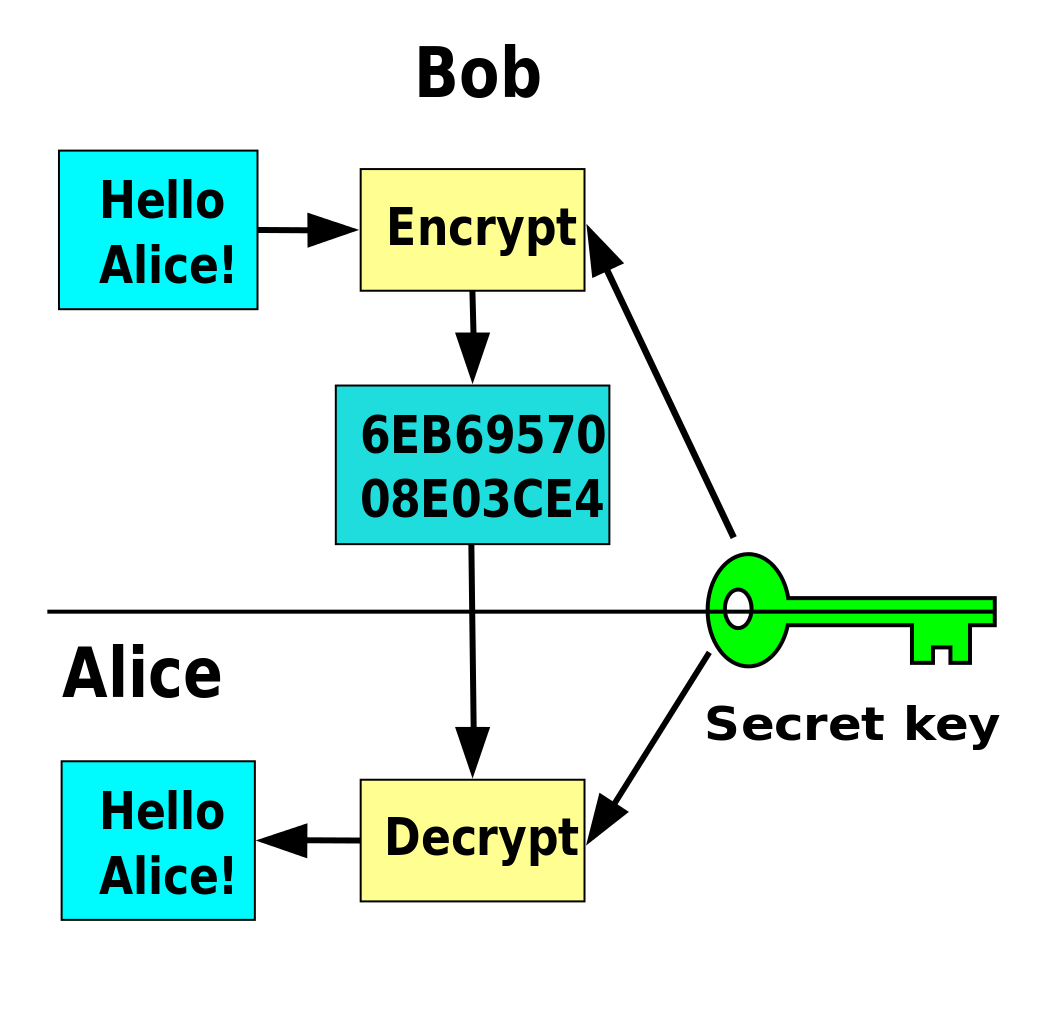
\includegraphics[scale=0.25]{./SymmetricKey.png}
					\caption{Symmetric Key Cryptography Process}
					\label{fig:SymmetricKey}
				\end{figure}
				The following steps are involved in communicating with this type of cryptography:
				\begin{enumerate}
					\item Alice and Bob agree on a Cryptosystem. 
					\item Alice ad Bob agreed on a key. 
					\item Alice encrypts the plaintext message. 
					\item Alice Sends the ciphertext to Bob. 
					\item Bob Decrypts and reads the message.
				\end{enumerate}

				Eve, an attacker against this system could attack at step 4, requiring a ciphertext-only attack. 
				However, this would likely not work as current cryptography standards are resilient to this given modern compute power. 
				Rather than hope a poor method of encryption was used, Eve would attack steps 1 and 2, 
				attempting to gain the same information about the key and algorithm as Bob has. 
				With this information, Eve would simply have to capture and decrypt the message as Bob would normally. 

				This presents the main problem with symmetric key encryption, \emph{key distribution}. 
				There are solutions to this, such as meeting face-to-face to pass the key from Alice to Bob or 
				using public key cryptography, as explained later in this chapter. 

				There are also further issues when you account for an active attacker, Mallory. 
				Mallory could simply block communications, or could replay communications in an attempt to illicit a reaction. 
				Further, Mallory could capture the key as explained above and impersonate Alice, passing malicious messages that would seem to come from her. 
				In these cases, there is no way for Bob to know that the messages are coming from Mallory rather than Alice. 

				Finally, there are some impracticalities with this system. 
				If a different key is used between every pair of members on the network, the number of keys grows rapidly. 
				A network of $n$ users requires $\frac{n(n-1)}{2}$ keys. 
				For a network of only 100 users, there would be 4950 keys. 
			\subsection{One Way Functions}
				One way functions are the foundation of public key cryptography, explained in the following section. 
				The functions have not been mathematically proven, but computationally have been found to exist. 
				The premise is that they are easy to compute it one direction, but hard to return from. 
				That is, given $x$ it is easy to compute $f(x)$, 
				however, given $f(x)$ it is hard to the point of infeasibility to compute $x$. 

				An example of this, left to the reader to conduct is that of a message written on a plate:
				\begin{enumerate}
					\item Write a message, $x$ on a plate. 
					\item Throw the plate as hard as you can on a hard surface, shattering it. 
						This acts as $f(x)$. 
					\item Give the plate to a friend, asking them to tell you the message, $x$. 
				\end{enumerate}

				A simple one way function is not useful for public key cryptography, 
				something more, known as a trapdoor function is needed. 
				These functions are a special type of one way function that can be computed in reverse easily. 
				However, this process only works if given an extra piece of information. 
				These are fundamental to public key cryptography. 

			\subsubsection{Public Key Cryptography}
				Unlike symmetric key cryptography, public key cryptography uses two keys, one stored at each party. 
				These two keys are completely different. 
				They are designed in such a way that given one of them, you should not be able to determine the other. 

				These two keys each have a name and a set of properties. 
				The key used to encrypt the data is known as the public key. 
				It can be read by anyone, as it will not give them access to the data. 
				The key used to decrypt the data is known as the private key. 
				This key will be securely stored on the receiving computer and should never be transmitted. 
				While this solves the problem of key exchange, it is significantly slower. 
				An example of this process can be found in figure \ref{fig:PublicKey}
				\begin{figure}[htb]
					\centering
					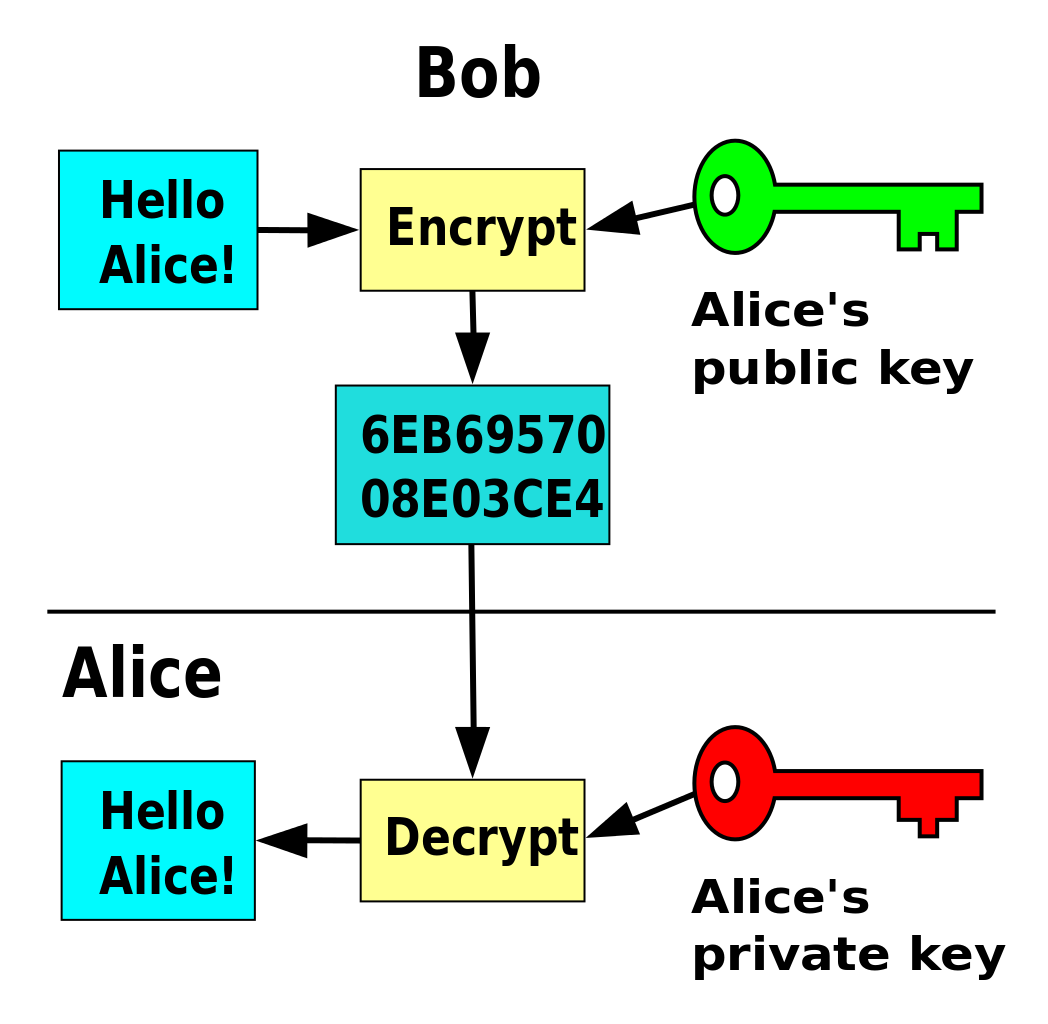
\includegraphics[scale=0.25]{./PublicKey.png}
					\caption{Public Key Cryptography Process}
					\label{fig:PublicKey}
				\end{figure}

				This process is similar to having a locked mailbox. 
				Anyone can place mail in the box (encrypting it and sending it to you). 
				However, it is exceptionally difficult given the mail slot alone to open the box and access the mail. 

				Mathematically, this is based on the trapdoor one-way function discussed above. 
				Encrypting the message is the easy direction, meaning that anyone with the public key can encrypt and send messages.
				Decryption however, is in the hard direction. 
				The secret here is the private key. 
				Using this, one can decrypt the message easily. 
				Without it, the message remains a secret. 

				The process involved in public key cryptography is as follows:
				\begin{enumerate}
					\item Alice and Bob agree on a public key cryptosystem. 
					\item Bob sends Alice his public key. 
					\item Alice encrypts her message using Bob's public key and sends it to Bob. 
					\item Bob Decrypts Alice's message using his private key. 
				\end{enumerate}

				This process resolves the problem of key distribution seen above in secret key cryptography. 
				While Bob must in step 2 send his public key in plaintext, Eve cannot read any messages using this key. 

				There are however still problems with this system. 
				Public key algorithms are significantly slower than symmetric key algorithms, often at least 1000 times slower. 
				This places strain on the bandwidth which can be processed by a computer. 

				Furthermore, these system are more vulnerable to chosen-plaintext attacks. 
				As the encryption key is known, an attacker can encrypt all possible plaintexts in a similar way to rainbow tables as explained below under hash cracking. 
				While this attack will not show the key, it makes it trivial to use deduce any plaintext from any ciphertext. 

			\subsubsection{Hybird Cryptosystems}
				These systems were built to use the better of both symmetric and public key cryptography in any given circumstance.
				They will choose the necessary system to use their advantages but minimize their disadvantages. 

				The main example of this is the exchange and use of session keys. 
				In this scenario, public key encryption is used to transport a randomly generated session key. 
				From this point on, symmetric key encryption is used as it is faster and less vulnerable to attacks. 
				In this example, the process for communication is as follows:
				\begin{enumerate}
					\item Alice and Bob agree on a public key cryptosystem and a symmetric key cryptosystem. 
					\item Bob sends Alice his public key. 
					\item Alice generates a random session key, encrypts it using Bob's public key and sends it to Bob. 
					\item Bob decrypts this key using his private key, recovering the session key. 
					\item Both Alice and Bob begin communicating over a symmetric cryptosystem using the shared session key. 
				\end{enumerate}
				
			\subsubsection{Hashing}
				Hashing does not involve a key, though it may use a salt to ensure the uniqueness of the hash. 
				This process creates a fixed length hash value which represents the plain text message. 
				However, there is no way of taking this hash value and algorithmically decoding the plain text from it. 

				This process is often used in checking that the correct data was transmitted unaltered. 
				It can further be used for the storage of items that need to be checked but should not be stored in plain text. 
				An example of this would be the storage of passwords. 
				
				An example of the hashing process can be found in figure \ref{fig:HashingProcess}
				\begin{figure}[htb]
					\centering
					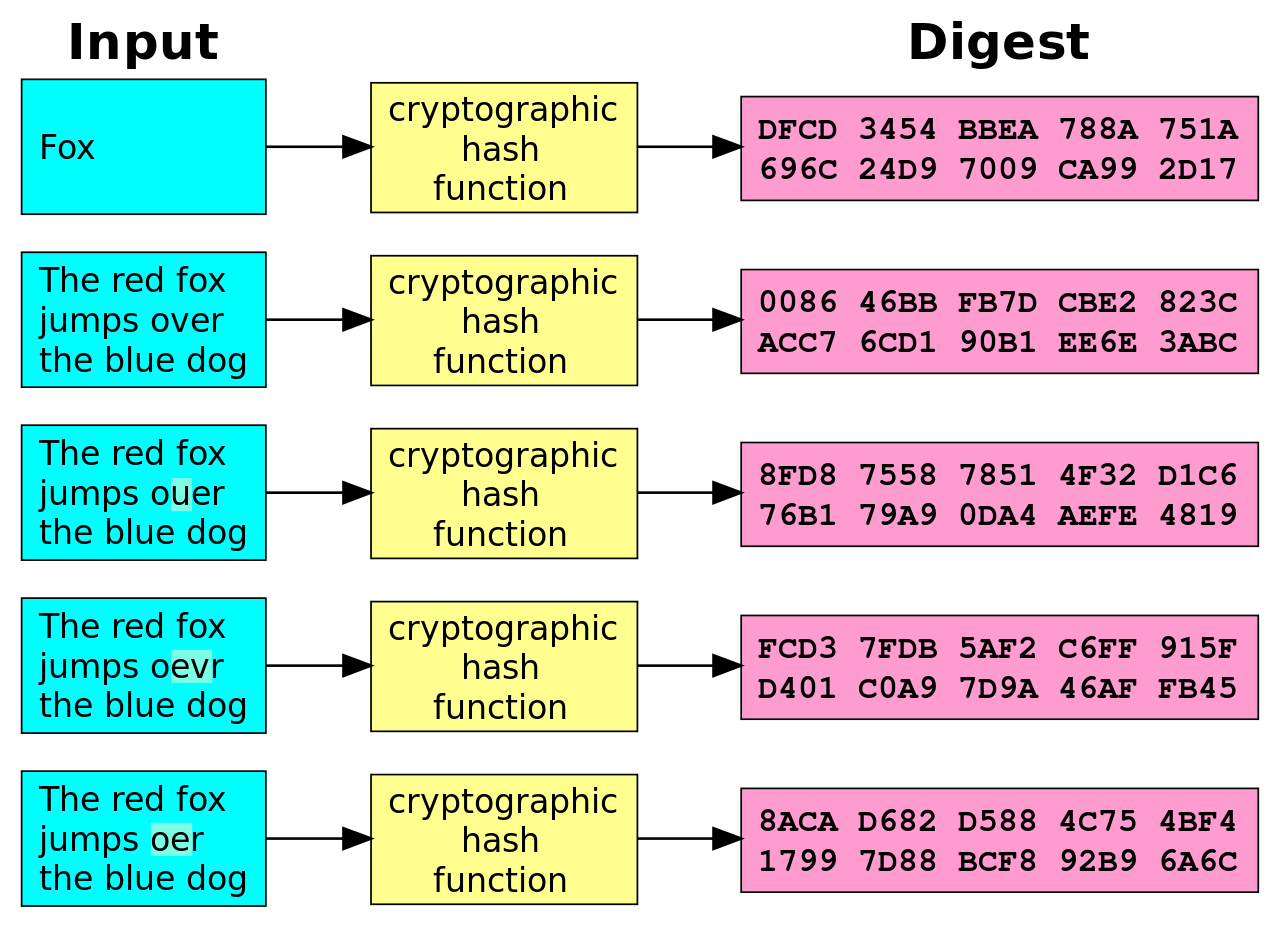
\includegraphics[scale=0.25]{./HashProcess.png}
					\caption{Hashing Process}
					\label{fig:HashingProcess}
				\end{figure}

				The security of a hashing function is found in the one-wayness. 
				This means that it cannot be used to compute the original value. 
				Furthermore, a hash function that is collision-free is far more secure that one for which it is easy to compute two values that output the same hash. 

			\subsubsection{Algorithmic Security}
				The algorithm used to conduct cryptography is the modern world should be considered accessible to anyone. 
				This is due to the simple fact that the program used to implement the algorithm can be reverse engineered by any significantly motivated party. 
				Once the program is reverse engineered, the algorithm is freely known to that party. 

				Due to this, one must remember not to trust any hidden algorithm. 
				These are likely to be un-reviewed, leaving large holes in their implementation unnoticed. 
				Furthermore, any security provided by hiding the algorithm will be undone purely through the use of reverse engineering. 
				As such, private algorithms should be considered snake oil until they are publicised and reviewed. 

				Further to this, the security of any algorithm should be considered before implementation. 
				For example, if your data is not exceptionally important, it will likely be secure with a lesser algorithm purely because the cost of breaking it outweighs the value of the data. 
				Furthermore, if the data is only sensitive for a short time, the data is secure as long as it takes longer than this time to break the algorithm for your current key. 

				It is also worth noting that there are two different types of security in algorithms:
				\begin{enumerate}
					\item Unconditionally secure: No matter how much of the ciphertext the attacker has, they will not be able to deduce any keys or plaintext. 
						The only system which meets this requirement is the one-time pad, which will be explained later in this chapter. 
					\item Computationally secure: The algorithm is computational infeasible to break. 
						This means that it requires far too much compute power or time to break, making the plaintext either less valuable or outdated by the time it can be retrieved. 
				\end{enumerate}
				In the former case, the algorithm is secure unless a cryptographical flaw can be found. 
				However, in the latter case, the algorithm is only secure given the current state of compute power. 
				If this were to increase substantially---which it currently is---the algorithm may no longer be secure in the given time frame. 

		\subsection{Basic Cryptography}
			Cryptography has been around since ancient times. 
			However, it has only been with the introduction of the modern computer that it has become complex and of a high standard. 
			This is because computers are good at breaking weak cryptography, that was the whole purpose of the first digital computer created by Alan Turing and his team at Bletchley Park. 
			This first machine was designed to break the German Enigma Code and was exceptionally successful at it. 

			Basic encryption should not be used in the modern world. 
			It is not the type of encryption that would survive seconds against a well programmed computer. 
			Rather, it is the type of encryption that worked well for the Romans on the battlefield, well before the other commanders had heard of such techniques. 
			Many of the implementations seen in this area were based on characters within the text, 
			rather than the current workings which act on the binary of the message. 
			However, the same ideas form the foundations of modern cryptography in a more complex implementation. 
			If you would like to read further into these older forms of cryptography, I suggest Singh's \textit{The Code Book}\cite{CodeBook}.
			
			This section will first discuss the basic types of encryption that have been used---and still form the basis of modern cryptography. 
			It will then discuss some simple examples of old or defunct cryptographic standards.

			\subsubsection{Substitution Ciphers}
				This is an algorithm in which each acharacter in the plaintext is substituted with a corresponding one in the ciphertext. 
				The receiver then inverts this process when attempting to decrypt to plaintext. 
				There are a number of basic types of substitution cipher:
				\begin{description}
					\item[Simple] Each character is replaced with a corresponding character of ciphertext. 
					\item[Homophonic] Similar to Simple Ciphers, except a single plaintext character could correspond to multiple ciphertext characters. 
						For example, `a' could correspond to `15', `6' or `23'. 
					\item[Polygram] Blocks of characters are encrypted in groups. 
						For example, ``ARA'' could correspond to ``RLT''. 
					\item[Polyalphabetic] Made up of multiple simple substitution ciphers. 
						There may be multiple runs with different ciphers, or a different cipher may be used based on character position. 
				\end{description}

				Examples of these such as the Caesar's cipher are discussed below. 
				However, these are not commonly used today, outside areas such as hiding solutions to puzzles or spoilers in UNIX chat rooms. 

				The main vulnerability of this type of cipher is it's inability to hide the frequency of letters used in the plaintext. 
				Generally, this is exploited by statistically analysing the frequencies of characters used in the text. 
				It is likely that the most common characters will correspond to vowels, while the most common will correspond to `E'. 
				Such an analysis done on plaintext can be seen in figure \ref{fig:LetterFreq}
				\begin{figure}[htb]
					\centering
					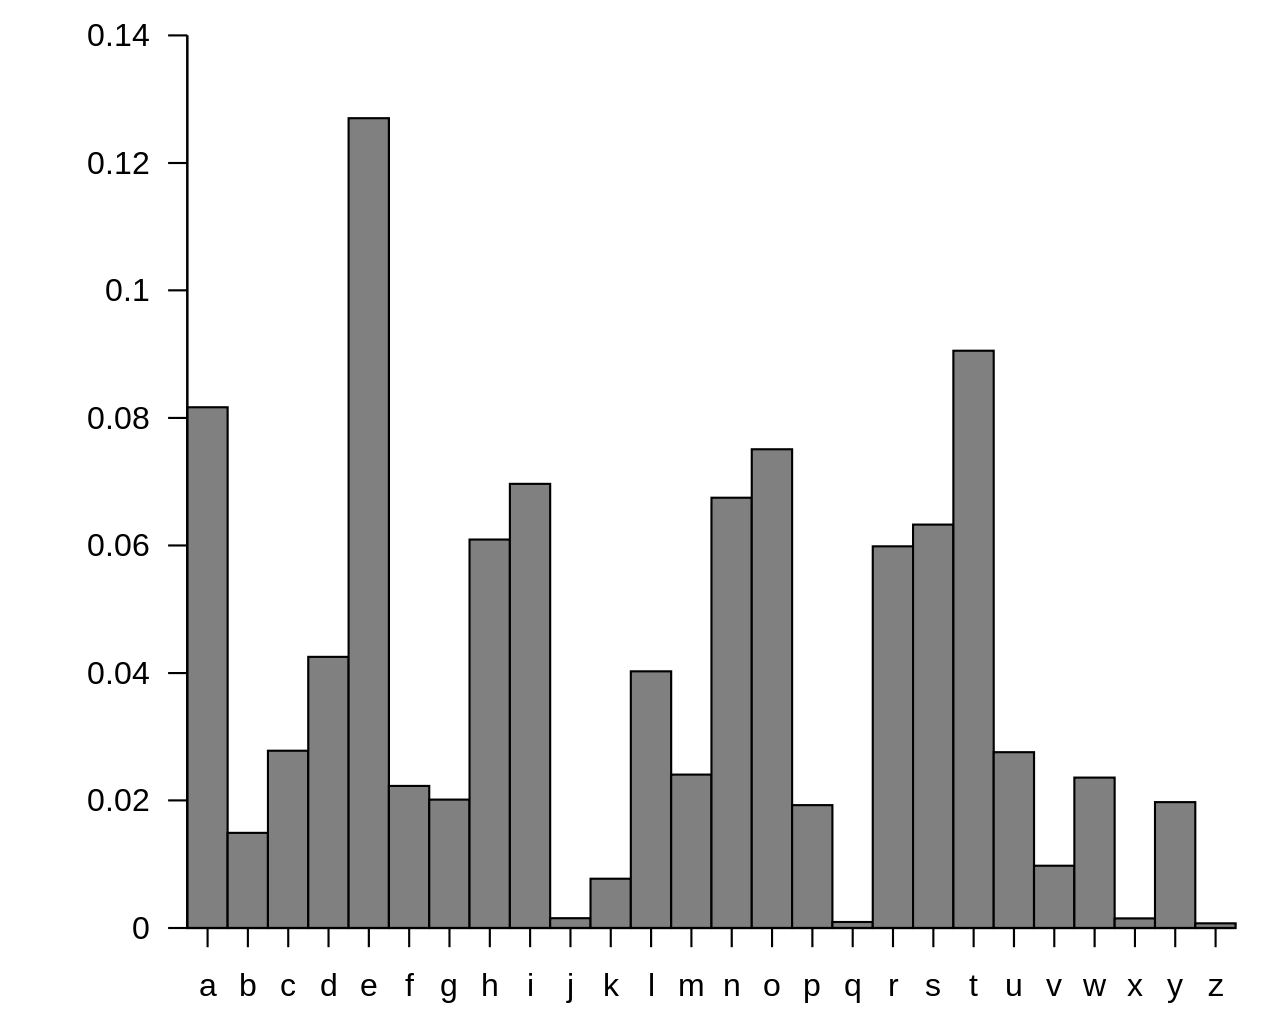
\includegraphics[scale=0.2]{./letterFreq.png}
					\caption{Frequency Analysis of Letters used in English Plaintext}
					\label{fig:LetterFreq}
				\end{figure}

				Due to this, the Homophonic Substitution Cipher was created. 
				This cipher effectively combats the issue of frequency analysis by allowing one character to map to many. 
				Thus, looking for the most common characters in the ciphertext will not lead you to the most common character in the plaintext. 
				However, this cipher is still exceptionally vulnerable to known plaintext attacks due to the ease of mapping character positions. 
				Furthermore, a ciphertext only attack can still be done using the correct algorithm in seconds on a computer. 
			\subsubsection{Transportation Ciphers}
				In this cipher, the plain text remains the same, but the location of the characters within it are changed. 
				An example of this is the simple columnar transportation cipher discussed below. 

				When analysing this type of cipher, the most obvious result that you will get is that the frequency analysis will be the same as a standard English text. 
				This is because none of the characters are changed, resulting in the same frequency but garbled text. 
				Once this is known, analysis and algorithmic attacks are generally quickly successful. 

				This type of cipher is far less common in modern cryptography as it requires large amounts of memory
				and sometimes requires that the messages be of a specified length, resulting in padding or split messages. 
			\subsubsection{Caesar's Cipher}
				This is the first algorithm that we will discuss. 
				It has little current use, as it's keyspace is 25, however, it serves as a good learning tool. 

				Caesar's Cipher is a simple substitution cipher\footnote{\url{http://www.pgpi.org/doc/pgpintro/}}. 
				This means that the key is simply a number that the alphabet used is shifted by. 
				Then, each letter in the plain text is substituted for the equivalent letter in the shifted alphabet. 
				This process can be seen in figure \ref{fig:CaesarsCipher}
				\begin{figure}[htb]
					\centering
					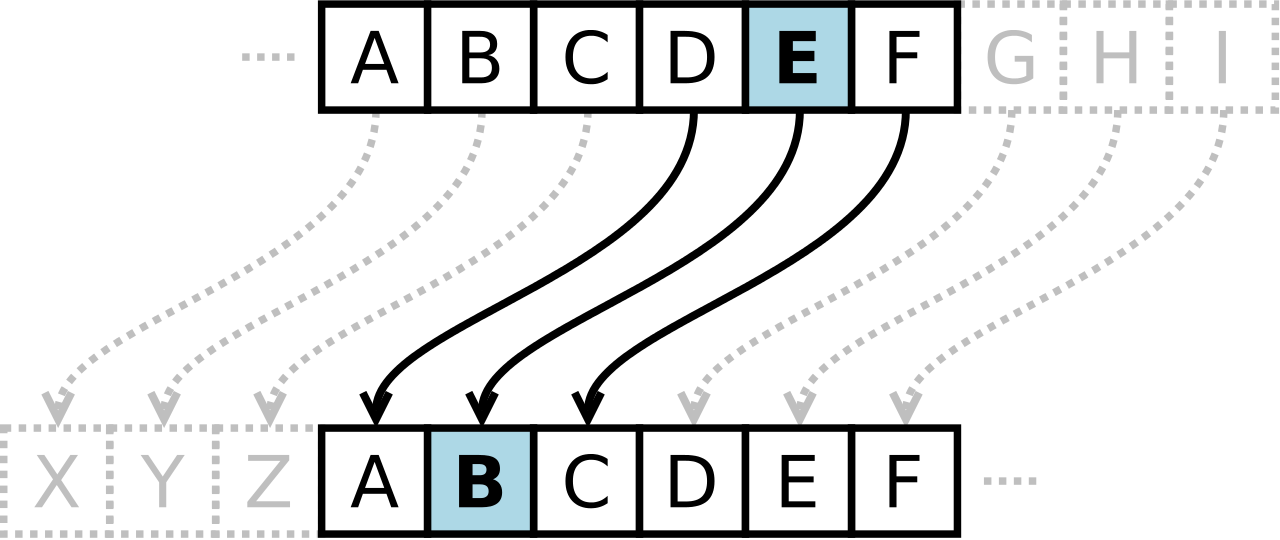
\includegraphics[scale=0.25]{./CaesarsCipher.png}
					\caption{The Method used for a substitution cipher}
					\label{fig:CaesarsCipher}
				\end{figure}
			\subsubsection{Columnar Transportation Cipher}
				This cipher simply moves the characters found within the plaintext to another location. 
				Specifically, the columnar transportation cipher uses a number as the key, which defines the number of rows to count.
				The plain text is then written out in rows of the length given by the key. 
				Plaintext will be written out horizontally, ciphertext will be read vertically. 
				This process can be seen in figure \ref{fig:ColumnarTransportation}.

				\begin{figure}[htb]
					\centering
					\begin{tabular}{|c|}
						\hline
						\textbf{Plaintext:}  WE ARE DISCOVERED. FLEE AT ONCE \\ 
						\texttt{W\,E\,A\,R\,E\,D} \\
						\texttt{I\,S\,C\,O\,V\,E} \\
						\texttt{R\,E\,D\,F\,L\,E} \\
						\texttt{E\,A\,T\,O\,N\,C} \\
						\texttt{E\thinspace\hphantom{A\,T\,O\,N\,C}}	\\
						\textbf{Ciphertext:} EVLNA CDTES EAROF ODEEC WIREE \\ 
						\hline
					\end{tabular}
					\caption{Example of Colunmar Transportation Cipher}
					\label{fig:ColumnarTransportation}
				\end{figure}

			\subsubsection{XOR Cryptography}
				In the same light as the Caesar's cipher, XOR should not be used when you are looking for security. 
				However, it is a stronger algorithm than the substitution cipher shown above. 
				This is due to the fact that the key which can be used for XOR can be as long as the plain text. 

				XOR is actually just a binary form of a Vign\`{e}re polyalphabetic cipher. 
				However, it is prevalent in a number of software packages and can be useful in hiding data from systems such as anti-virus. 

				While stronger than a substitution cipher, XOR still has a number of issues. 
				Foremost is the fact that it is easily reversible. 
				This means that given a known part of the plain text, the key can be deduced. 
				This becomes most obvious when the plain text has a section of null bytes. 
				These bytes will output as the key when passed through the algorithm. 
				Thus, if the attacker may know any part of the plain text, or can control it, XOR is just as weak as a substitution cipher. 

				Furthermore, there is no key chaining done in this algorithm. 
				Thus, if a short key is used, common parts of the plain text will be output in a similar way. 
				This means that images could still show detail and the cipher text is vulnerable to statistical analysis. 

				The XOR algorithm works by running a binary exclusive OR (see chapter \ref{ch:GeneralKnowledge}) 
				over each bit within the plain text and key. 
				The key is looped around, such that each time it gets to the end it links back to the start. 

				\begin{figure}[htb]
					\centering
					\begin{tabular}{| l | l | l |}
						\hline
						\textbf{Plaintext} & \textbf{Key} & \textbf{Ciphertext} \\ \hline
						10101011101010 & 10101110 & 00000100111101 \\ \hline
						00000000000000 & 10101110 & 10101110101011 \\ \hline
						10101011101010 & 00000000 & 10101011101010 \\ \hline
					\end{tabular}
					\caption{XOR Cryptography Example}
					\label{fig:XORExample}
				\end{figure}
				The process to break XOR is as follows:
				\begin{enumerate}
					\item Use ``counting coincidences'' to find the key length. 
						This is done by XORing the ciphertext against itself shifted by various numbers and counting the bytes which are equal. 
						If the displacement is a multiple of the key length, more than 6\% of the bytes will be equal, assuming ASCII plaintext. 
						This is called the \emph{index of coincidence}, the smallest of which is the key length. 
					\item Shift the ciphertext by the index of coincidence and XOR it with itself. 
						This removes the key from the ciphertext, leaving the plaintext XORed wit the plaintext shifted by the length of the key. 
						Using general cryptanalysis after this point will retrieve the plaintext. 
				\end{enumerate}

			\subsubsection{Encodings}
				Many people confuse encoding for encryption. 
				This confusion can lead to information being leaked, as encoding will not provide any protection. 
				To the untrained eye, these two look similar. 
				However, there are differences that should be understood and can be used to detect which is being used. 

				Encoding, much like encryption and hashing uses a known algorithm. 
				However, unlike encryption, encoding does not use a key. 
				Furthermore, unlike hashing, encoding is not one way. 
				This means that encoding can quickly and easily be returned to plain text as the means of returning is embedded within the algorithm.

				Encoding works by specifying a known character set and mappings amongst this. 
				For example, the binary data that forms this document in encoded as UTF-8, which you read as text. 
				However, this can be done in a different manner. 
				For example, this text could be encoded as a number, or as base 64. 

				Each of these different types of encoding has some part which can be used to determine what type of encoding is used. 
				For example, simple text will usually be encoded as ASCII. 
				Higher characters will have to be encoded as UTF-8 or UTF-16. 
				Numbers can be encoded as decimals, or in a higher base such as 16 or 64. 
				Table \ref{tab:Encodings} contains a list of the names and look of many common encodings. 
				\begin{table}[htb]
					\centering
				\begin{adjustbox}{max width=1\textwidth}
					\begin{tabular}{| l | l |}
						\hline
						\textbf{Name} & \textbf{Encoded Text Example} \\ \hline
						ASCII, UTF-8 etc & This is normal text \\ \hline
						Hexadecimal, base 16 & DEADBEEF, 46DEAC46BC \\ \hline
						Base 64 & YW55IGNhcm5hbCBwbGVhcw== \\ \hline
					\end{tabular}
				\end{adjustbox}
					\caption{Common Encoding Examples}
					\label{tab:Encodings}
				\end{table}
	\section{RSA}
		
		\subsection{\{N : e : c \} Format}
		\subsection{Common Flaws}
		\subsection{Key Recovery}
	\section{One Time Pad}
		As discussed above, this is the only perfect cryptographical implementation we have found to date. 
		This algorithm---discovery of a fatal flaw permitting---cannot be cracked by any computer in any amount of time. 

		The one time pad works by creating a sequence of random data as long as the message for the key. 
		This same key must be sent to the receiver so the message can be decrypted. 

		Using this, the sender will encrypt one plaintext character with one key character in the following manner:
		$$ (P + K) \bmod{26} = C $$  
		Where:
		\begin{description}
			\item[P] is the plaintext character. 
			\item[K] is the key character.
			\item[C] is the ciphertext character.
		\end{description}

		Assuming the key is sent with no way to intercept it, this system is perfectly secure. 
		That is, a given ciphertext message is equally likely to correspond to any plaintext. 
		This is because the key is random, non-repeating and replaced at every character. 
		Thus, any attempt to analyse the ciphertext will lead to the realisation that no information about the plaintext is provided.

		However, no matter how secure the algorithm itself it, if the input is not valid, it can be broken. 
		The largest flaw in this system is that it requires the key to be generated randomly, which is difficult to do on a deterministic computer. 
		
		Furthermore, the key cannot be reused. 
		If it is, breaking the cipher becomes a matter of sliding a pair of ciphertexts along one-another until the proportion of matches jumps suddenly. 
		At this point, breaking the cipher becomes similar to the XOR function discussed above. 
		One need only work with two ``periods'' rather than the previous incidence of coincidence. 

		This same solution works with binary on a computer. 
		A plaintext is generated and converted to binary, as is a random key.  
		The two are then XORed together, creating a random ciphertext. 
		The security of this system remains exactly the same, with both the same absolute security and possible flaws. 

		There is another large issue with this system. 
		It requires that both the sender and receiver have the same random key, at the exact length of the message. 
		This is fine for small messages, but becomes impossible for large ones. 
		For example, downloading a multi-gigabyte file using this would require the transfer of multi-gigabyte keys first. 

		These issues mean that one-time pads are not commonly used for civil computing. 
		It has been rumored that devices such as the cold war hotline between the US and USSR was encrypted using this. 
		Similarly, some messages to and from government agents during this time were encrypted using one-time pads. 
		However, it is unlikely to be used in anything but the most secure, low bandwidth communication channels. 
		Thus, the absolute security of the one-time pad becomes a thing of dreams again. 
	\section{Digital Signatures}
		Signatures on documents have been used in some form since ancient times. 
		They were used to ensure that the person you expect wrote or agrees with the document. 
		Furthermore, they were expected to be unforgeable, unmovable and irrefutable. 
		However, in practice, none of these things have been found to be true. 

		This is further exacerbated by computing. 
		An image of a signature inserted into a document is trivial to lift from that document and place anywhere else. 
		Furthermore, it is generally easy to edit a document after it has been signed. 
		Thus, a means of cryptographically signing the document must be created if authenticity and irrefutability are to be retained. 

		\subsection{Symmetric Signing with an Arbitrator}
			One way to authentically sign a document to give to another person or computer is to use an arbitrator. 
			In the physical world, this is similar to using a witness. 
			However, unlike in the real world, this arbitrator must be permanently trusted with the document. 

			Before starting, Alice and Bob need to be given permanent secret keys by Trent (The arbitrator). 
			These keys will be referred to as $K_A$ and $K_B$ respectively. 
			The process for signing is as follows:
			\begin{enumerate}
				\item Alice encrypts mer message to Bob with $K_A$ and sends it to Trent. 
				\item Trent decrypts the message with $K_A$. 
				\item Trent takes the decrypted message, adds a statement that he has recieved this message from Alice, encrypts the new message with $K_B$.
				\item Trent sends the encrypted message to Bob. 
				\item Bob decrypts the message with $K_B$. He now reads the message and the certification that Alice was the sender.
			\end{enumerate}

			This system works. 
			It removes the issues described above with physical signatures, while working on a computer network. 
			However, it is time consuming for the arbitrator, and requires that each user have a key that is permanently stored and reused. 
			Furthermore, creating a trusted middleman in all communications creates a single point of failure, both in security and in function. 

		\subsection{Public Key Signatures}
			To solve these problems, public key signatures were created. 
			These work using an algorithm such as RSA in the reverse manner to it's creation:
			\begin{enumerate}
				\item Alice encrypts the document with her \emph{private key}.
				\item Alice sends the document to Bob. 
				\item Bob decrypts the document with Alice's \emph{public key}. 
					This verifies that the document was sent by Alice. 
			\end{enumerate}

			This protocol removes a number of the previous issues. 
			While Trent is still necessary to verify that the correct public key for Alice is being used, he is not needed for communication or dispute resolution. 
			This reduces stress on the network, and removes most of the large single point of failure from the previous model. 

			There is however, a significant issue here. 
			Bob can choose to replay the message sent to him to anyone else on the network. 
			This isn't a problem if the message is a contract. 
			However, if the message is a digital cheque or other means of payment, Bob can now replay this message, stealing money from Alice. 
			Due to this, a public key signature will often contain a timestamp of the signing which is appended to the message. 
			An institution using the signed information would take note of the timestamp and check whether the same stamp had been used previously. 
			Thus, these messages can only be used once. 

			In practice, these signatures can be large and slow to generate. 
			To resolve this, we use a one-way hashing function on the document and sign the hash. 
			This means that the receiver need not store both the document and a signature at the same size. 
			Rather, they can store a 256-bit hash signature and the document. 
			Not only is this faster, it is also easier to store and just as accurate. 
			
		\subsection{Resend Attacks}
			Some systems will both sign and encrypt a message using the same keys and algorithms (RSA for example will do both). 
			Generally, this is useful, as it provides both security and authenticity. 
			However, when these systems implement receipts, they can become a security flaw. 
			Take the following example:
			\begin{enumerate}
				\item Alice signs a message with her private key, encrypts it with Bob's public key and sends it to Bob. 
				\item Mallory records this message in transit. 
				\item Mallory resends this message to Bob, claiming that it came from him. 
				\item Bob decrypts the message and attempts to verify it with Mallory's public key. 
					This results in pure gibberish. 
				\item Bob encrypts and signs the message and returns a receipt to Mallory. 
				\item Mallory then follows the following steps to gain the message:
					\begin{enumerate}
						\item Decrypt the message with his private key. 
						\item Encrypt the message with Bob's public key. 
						\item Decrypt the message with his private key. 
						\item Encrypt the message with Alice's public key. 
						\item Read the now plaintext message. 
					\end{enumerate}
			\end{enumerate}

			The solution to this, is first to check what the message is before sending a receipt, but also to use different keys or algorithms for signatures and encryption. 
			Alternatively, using digital signatures based on hash functions, rather than the whole document will solve this as the signing process is only done on the hash. 

	\section{Merkle-Hallman Knapsack Cryptosystem}
	\section{Key Exchange}
		%Resource: http://security.stackexchange.com/questions/45963/diffie-hellman-key-exchange-in-plain-english
		Getting assured access to other peoples public keys is not an easy task. 
		If they were to send it to you in plain text, it may be intercepted and altered. 
		Furthermore, in this scenario, signatures are pointless as anyone can impersonate another party by sending you a public key and telling you who they want to be. 

		This is solved by having a key distribution centre (KDC). 
		Such a system works by creating a public database of keys stored by a trusted party.
		This database contains both the public keys and names of individuals on the network. 
		Each public key is signed by the KDC, assuring the end user that it is a valid key. 

		Again however, this begs the question of how did Alice gain access to the KDC's public key?
		If Mallory could send Alice a false public key, they could act as the KDC themselves. 
		Similarly, Mallory could attack the large central target that is the KDC, giving them access to create a false key for anyone. 

		This system relies on trust and making this harder than it is worth. 
		It is still far better than physical signatures and with a well secured KDC, it can be exceptionally difficult to break. 
	\section{Server Authentication}
	\section{Rotational Algorithms}
	\section{Utilizing Cryptography in Python}
	\section{Poor Cryptography Implementations}
		\subsection{DES Weak Keys}
	\section{Eilliptic Curve Encryption}
		\subsection{Common Attacks}
	\section{Hash Cracking}
		Hashes are used in many situations to store passwords. 
		This is done because the hashing algorithm is a one way action, meaning that there is no easy way to calculate the password from the hash. 
		Due to this, the means of authentication on most programs is done by hashing the entered password and comparing it to a stored hash. 
		If the two match, it is likely---though not guaranteed due to collisions---that the password is the same. 
		While this may sound like it makes attacking these targets hard, it is far from being unsolvable. 
		Tools such as ``John the Riper'' and ``Hashcat'' can be used to compute hundreds of thousands of hashes per second, which can then be compared with the given hash. 
		This makes hash cracking a matter of time and dictionary crafting. 
		\subsection{John the Riper}
			While there are many tutorials\footnote{\url{http://openwall.info/wiki/john/tutorials}} on the usage of John the Riper (John) which go into specific detail, this section will explain the basic usage of the tool. 
			Before starting, check that the version of John which you have installed is correctly compiled for your system, you may want to enable options such as GPU cracking, which needs to be done at compile time. 
			What follows is a list of common commands for use with John:
			\begin{description}
				\item[-single]
					The simplest means of attacking a hash. 
					This mode uses only a basic word-list and very few rules. 
					Thus it is not recommended for anything but the most basic attacks. 
				\item[-wordfile:]
					Uses the word-list specified directly after the colon. 
				\item[-rules:]
					Specifies the mutation rules for the given word-list. 
					These can be used to create a dictionary with substitutions, such as 1337 speak. 
				\item[-incremental:]
					This, along with options such as ``alpha'', ``digits'' or ``lanman'' will give you a brute force of letters, numbers or both with some special characters respectively. 
				\item[-external:]
					Allows the use of pre-configured modes, which can be powerful if used or modified correctly. 
					%TODO: add more to this and rules. 
				\item[-restore:]
					Will start a crack part way through based on a restore file created by a previous session. 
				\item[-sesion:]
					Used to name the restore file that will be created when the session is broken. 
				\item[-status:]
					Shows how far into the crack a previous session was stopped. 
				\item[-show]
					Shows how many passwords within a file have been cracked and how many remain. 
				\item[-format:]
					Specify the hash format (such as SHA512) which the hash to crack was created with. 
			\end{description}
			
		\subsection{Hashcat}
			Hashcat was started due to the fact that at the time, tools such as John the Riper did not make proper use of multi-threading. 
			This has been expanded to include GPGPU processing using tools such as openCL and CUDA, and has made hashcat one of the fastest hash cracking tools currently available. 
			Both Hashcat and the newer oclHashcat use the same input files and command syntax. 
			However, oclHashcat will conduct the crack on the GPU installed on the system, rather than the slower CPU. 

			Hashcat uses a number of modes to allow it to crack hashes. 
			Each of these modes has a number of specific properties which make it better at a given type of attack. 

			\subsubsection{Mask Attack}
				This attack, while similar to a brute force attack, uses a mask to reduce the possible character set of the attacks.\footnote{\url{http://hashcat.net/wiki/doku.php?id=mask_attack}} 
				Rather than run through every possible permutation of the character space for every character in the password, the mask attack requires that the user input some details of the characters within the password. 
				
				When using this mode, for each position within the password, we need to create a mask using either the character sets outlined in table \ref{tab:HashcatMaskCharSets} or a custom character set defined before starting. 
				\begin{table}[htb]
					\centering
				\begin{adjustbox}{max width=1\textwidth}
					\begin{tabular}{| l | l |}
						\hline
						?l & abcdefghijklmnopqrstuvwxyz \\ \hline
						?u & ABCDEFGHIJKLMNOPQRSTUVWXYZ \\ \hline
						?d & 0123456789 \\ \hline
						?s & <space>!"\#\$\%\&\verb!'()*+,-./:;<=>?@[\]\^_`{|}~}! \\ \hline
						%?s & Special Characters \\ \hline%TODO: Have this print the characters. 
						?a & \verb+?l?u?d?s+ \\ \hline
						?b & 0x00 - 0xff \\ \hline
					\end{tabular}
				\end{adjustbox}
					\caption{Hashcat Mask Mode Built in Character Sets}
					\label{tab:HashcatMaskCharSets}
				\end{table}
				Attacks in this mode are limited by the length of the mask given. 
				This means that if you give a mask with 8 character spaces, but have a password which is 6 characters long, you will be unable to crack it. 
				Due to this, the ``\verb+--+increment'' flag was created. 
				Furthermore, a list of standard character sets for multiple languages can be found in ``/usr/share/hashcat/charsets/''.

				Another means of creating this attack mode is to use a Hashcat Mask File. 
				These files contain a number of masks and the custom character sets which are used within them, in order to run attacks which are regularly repeated. 
				To use one of these files, run Hash cat with the arguments ``-a 3 <hash file> <mask file>''.

			\subsubsection{Dictionary Attack}
				In this attack, a dictionary or word list is created to be utilized within the attack. 
				This dictionary can either be one that you found on the system or one that was created specifically for the job. 
				Due to the limitations of this attack, it is recommended that it is either used with a specifically generated dictionary, which can be done by a program such as John the Riper or
				a can be manually written through the use of a python script. 
				This type of attack may be the first that you use, as it will likely be the quickest attack. 
			\subsubsection{Combinator Attack}
				In this attack, each word of a dictionary is appended to each word in a second dictionary. 
				This will catch many passwords which use two simple words, as long as the dictionary is well written. 
				However, if the dictionaries that you are using have already been enumerated in such a way, it will likely not produce useful results. 
				Furthermore, this attack will not run the words from each dictionary separately. 
				To use this attack, run the top command for GPU or the bottom command for CPU. 
				\begin{lstlisting}[style=CLI]
					$ oclHashcat64 -m 0 -a 1 <hash file> <dict1> <dict2>
					
					$ hashcat-cli64 -m 0 -a 1 <hash file> <dict 1 and 2>
				\end{lstlisting}
			\subsubsection{Hybrid Attack}
				This attack uses the concepts of both the combinator and mask attacks. 
				This means that you can specify a dictionary and have hashcat add the mask that you give to either the start or end of the word. 
				Using this means, you can easily run through passwords such as name and birth year combinations. 
				To conduct this attack, use the command:
				\begin{lstlisting}[style=CLI]
					$ oclhashcat -a 7 <mask> <dict>
					$ oclhashcat -a 7 <dict> <mask>
				\end{lstlisting}
				
		\subsection{Rainbow Tables}
			In both of the previous sections, we have been calculating the hashes which we are testing against the password hash on the go. 
			This means that we have to calculate the algorithm, sometimes multiple thousands of times, for each password we want to try. 
			There is another option: rainbow tables. 
			This method of cracking passwords allows us to have a precomputed list of hashes and their respective passwords, which we then simply search through. 
			This results in two significant differences:
			\begin{itemize}
				\item Password cracking takes seconds
				\item Your hard drive is full. 
			\end{itemize}
			However, these tables are not the be all and end all of hash cracking. 
			They rely on the hashes being computed either with no salt or with the same salt as the table, meaning that hashes generated using a randomized salt will not be vulnerable. 
			Furthermore, they rely on the attacker being able to find a table which will suit the password. 
			Thus, if your password is a 50 character essay with special characters, it will likely not show up in the table due to size constraints. 
			Such a table would have to contain $\approx2.49\times10^{66}$ password--hash pairs, resulting in a file size of $\approx2.6\times10^{44}$Yottabytes.
			Though this cannot be thought of as a limitation when compared to the two other methods, as for the same password, they would take $\approx5.2\times10^{52}$ years on 3 ATI HD7970 GPUs.\footnote{\url{https://litecoin.info/Mining\_Hardware\_Comparison}}
			At this point, even assuming Moore's law continues and Processing power becomes far cheaper, the password will not be cracked within a reasonable time frame. 

			It is for these reasons that rainbow tables are uncommonly used outside of cracking hashes from poorly implemented software with short passwords. 
			However, if you know that the character space is small, and either the passwords are unsalted or the salt is commonly known, rainbow tables are the best method if you have the storage space. 
		\subsection{Online Methods}
			With the rise of cloud computing and cheap server rental, many people have begun using tools such as Amazon Web Services to run crack servers. 
			This is done by deploying the tools shown above into a server which has been rented with multiple GPUs. 
			This server can then be optimized such that the cracking will properly utilize the GPUs of the machine as well as only calculating hashes that have a possibility of being correct. 
			Thus, as above, if you know that the hash will be within a given dictionary, or that it does not contain special characters, use these functions. 

			While this will work, and usually faster than using one's own computer, it is not as fast as a dedicated cracking cluster. 
			These clusters work by having a number of machines, each with the necessary hardware and software installed working together on the one hash. 
			Programs such as Hashcat can be used to control up to 125 GPUs across the cluster in order to crack the hashes you provide. 
			This method, while expensive and difficult to set up, is currently the fastest means of cracking a hash. 
			However, if you set your cracking program up properly, it will still likely beat this setup when it is brute forcing hashes. 
		\subsection{Salting}
			Many of the methods above become significantly more difficult when salting is introduced. 
			Normally, a hash will be produced by simply running a hash function on the password ($hash(pass)$). 
			However, when salting is implemented, the hash may be generated by adding either a known string or a random string---or sometimes both---to the password before passing it to the hash function ($hash(pass + "salt"$ or $hash(pass + rand()$).
			In either of these cases, the salt must be stored, which has led to split salting, using a random stored value or the users name/ID as well as a hard coded element. 
			This makes knowing the salt hard, but not impossible, as we can reverse engineer the code in order to determine the salting algorithm used and a simple ``strings'' on the compiled code will give us a hard coded salt string. 
			Nonetheless, these methods deter attackers from attempting to crack the hashes by limiting their choices and removing their ability to use rainbow tables. 
		\subsection{SHA}
		\subsection{Hash Collisions}
			Hashes, by their nature must have collisions. 
			This is due to the fact that they take a large amount of information and turn it into a string of a standard size. 
			For example, an SHA256 hash has a length of 65 and a character space of 36. 
			This gives $1.84\times10^{66}$ possible values. 

			This is the basis for collisions. 
			Consider that there are vastly more than this number of items that can be hashed, 
			If this is true, some of these items must have the same hash value as other items.
			Furthermore, if you can find a collision with the item you are testing, you need only pass that collision, rather than the item itself. 

			This is the exact reason hashing algorithms such as MD5 are being replaced with SHA512. 
			It is now easy to find a collision value for the smaller key space MD5, meaning that using it for secure storage or any other purpose is near pointless. 

			Table \ref{tab:HashCollisions} contains the maximum number of hash values for common hash types.
			\begin{table}[htb]
				\centering
				\begin{adjustbox}{max width=1\textwidth}
				\begin{tabular}{| l | l |}
					\hline
					\textbf{Hash Type} & \textbf{Number of Values} \\ \hline
					SHA256 & $1.44\times10^{102}$ \\ \hline
					SHA512 & $5.79\times10^{201}$ \\ \hline
					SHA1   & $6.4\times10^{64}$ \\ \hline
					MD5	   & $2.28\times10^{52}$ \\ \hline
				\end{tabular}
			\end{adjustbox}
				\label{tab:HashCollisions}
				\caption{Number of Possible Hashes for Different Algorithms}
			\end{table} 
	\section{Challenges}
		\subsection{Hash Challenges}
			This first challenge is based on the \href{https://xkcd.com/936/}{xkcd comic ``Password Strength''.}
			The word-list for this challenge can be found by using the following command on kali linux:
			\begin{lstlisting}[style=CLI]
				$ head -n 20	/usr/share/wordlists/rockyou.txt
			\end{lstlisting}
			The password, hashed in MD5 and SHA256 can be found below. 
			\lstinputlisting[numbers=none,firstline=1,lastline=4]{./shellOut/hashChallenges.data}
			While you can complete this in any way you like, I recommend either using John's rules, or creating a custom word list and using Hashcat's hybird mode. 
			%Solution: "N1c0l3;7"

			The second challenge is based on an ATM keypad. 
			Through an image captured when the hash was pulled, it was determined that the only keys pressed were ``2, 4, 9 and 0''. 
			The password was also determined to be exactly 16 characters long. 
			Create a custom mask for Hashcat and solve this sha256 hash. 
			\lstinputlisting[numbers=none,firstline=6,lastline=6]{./shellOut/hashChallenges.data}
			%solution: "2490092442902942"

			The third challenge is based on using multiple dictionary words. 
			This is a common method used to create passwords. 
			I recommending using Hashcat in combinator mode to solve this SHA256 hash. 
			All the words necessary to solve this can be found in the rockyou word-list. 
			\lstinputlisting[numbers=none,firstline=8,lastline=8]{./shellOut/hashChallenges.data}
